%!TEX root = origin.TEX
\chapter{Introducción}
	\pagenumbering{arabic}
	\setcounter{page}{1}
	%\renewcommand{\baselinestretch}{2} %doble espacio paratodo el texto
	Al conducir en carreteras congestionadas, a veces es difícil mantener los ojos en todas partes a la vez, comprobando el camino por delante, el tráfico venidero, lo que está detrás de usted, tratar de mantener su velocidad; es por ello, que existen mecanismos destinados a reglamentar el tránsito, advertir o informar a los usuarios mediante palabras, sonidos o símbolos determinados. Un claro ejemplo de ello, es la policía de tránsito o las señalizaciones vehiculares que según sea el caso, en todos los países regulan el tránsito e informan al usuario sobre direcciones, rutas, destinos, así como dificultades existentes en las carreteras y previenen cualquier peligro que podría presentarse en la circulación vehicular.

	\vskip 0.15cm
	Sin embargo, cuando estos mecanismos no son conocidos o percebidos pueden ocasionar no solo que la congestión del tráfico aumente sino que también se produzcan accidentes que en muchos casos derivan en consecuencias fatales, generando inseguridad vial.

	\vskip 0.15cm
	La inseguridad vial es un problema de interés mundial, según el último informe de la OMS(Organización Mundial de la salud) anualmente cerca de 1,3 millones de personas mueren alredor del mundo y entre 20 y 50 millones padecen traumatismos no mortales,\citep{OMS}. Esto representa la segunda de las principales causas de muerte a nivel mundial entre los jóvenes de 05 a 29 años de edad, y la tercera entre la población de 30 a 44 años. Son distintas las causas que conllevan a este problema, de las cuales las principales pueden ser la falta de concientización y educación vial. 
	
	\vskip 0.15cm	
	Es un problema para la economía mundial de los países, así también para los hogares. A pesar de ello, se invierte muy poco dinero en prevenir los accidentes y las lesiones causadas por el tránsito. El sector salud se beneficiaría mucho de una mejor prevención de las lesiones porque se reducirían las hospitalizaciones y la gravedad de los traumatismos, \citep{CNSV}.

	\vskip 0.15cm
	Los usuarios vulnerables de la vía pública representan la mitad de todas las muertes por accidente de tránsito a nivel mundial y es mayor en países de ingresos bajos, siendo la causa principal el aumento de velocidad de los vehículos, \citep{OMS}.

	\vskip 0.15cm
	\begin{figure}[H]
	\begin{center}
	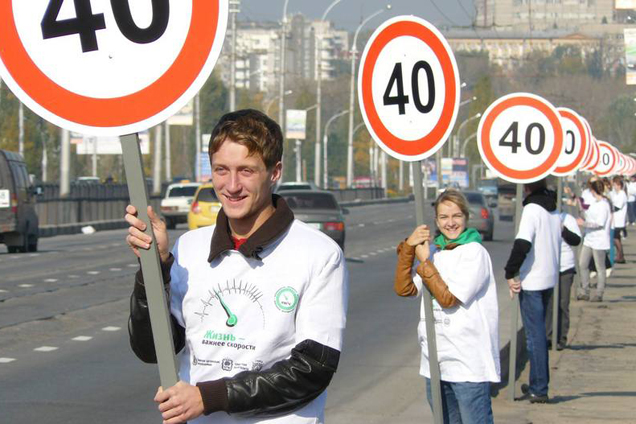
\includegraphics[width=0.75\textwidth]{images/intro/velocidad}
	\end{center}
	\begin{center}
	\caption{\small{Señalización de velocidad}}
	{\small{Fuente: \citep{OMS}}}
	\end{center}
	\vspace{-1.5em}
	\end{figure}
	
	Por otra parte, de los vehículos que se venden el 80\% de los países no cumplen las normas básicas de seguridad, es por ello que se debe trabajar en obtener vehículos más seguros ya que es un factor fundamental para prevenir de alguna forma los accidentes de tránsito o reducir la probabilidad de traumatismos graves en caso de que estos se produzcan, \citep{OMS}.
	
	\vskip 0.15cm
	En lo que respecta al sector local, es decir en el Perú, la inseguridad vial es un problema constante ya que los peruanos mueren más por los accidentes de tránsito que por la inseguridad ciudadana según datos mostrados por María Edith Baca de la Organización Panamericana de la Salud\citep{OPS}. Adicionalmente, según un estudio realizado por RPPData en base a reportes de la Policía publicados entre el 2010 y el 2016, en el país cada día fallecen 8 personas en accidentes de tránsito,\citep{RPPData}. El costo de estas muertes, calculado en S/ 19,165 millones por la consultora Alauda especializada en mantenimiento de infraestructura , representó un 3.1\% del PBI, \citep{Gestion2}.  
	
	
	\vskip 0.15cm
	En el 2016 se obtuvo un Índice Global de Satisfacción del Conductor \citep{CNN} en el cual, Perú y la capital Lima se encuentran respectivamente en la lista de peores países y ciudades para conducir en America Latina, esto se ve reflejado en que los últimos años se ha incrementado el índice de mortandad originados por los accidentes de tránsito siendo las principales causas de los mismos el exceso de velocidad, estado de ebriedad del conductor, imprudencia temeraria y el desacato a las señales de tránsito, todas ellas de responsabilidad directa del conductor del vehículo motorizado,\citep{SUTRAN}. 
	
	\begin{figure}[H]
	\begin{center}
	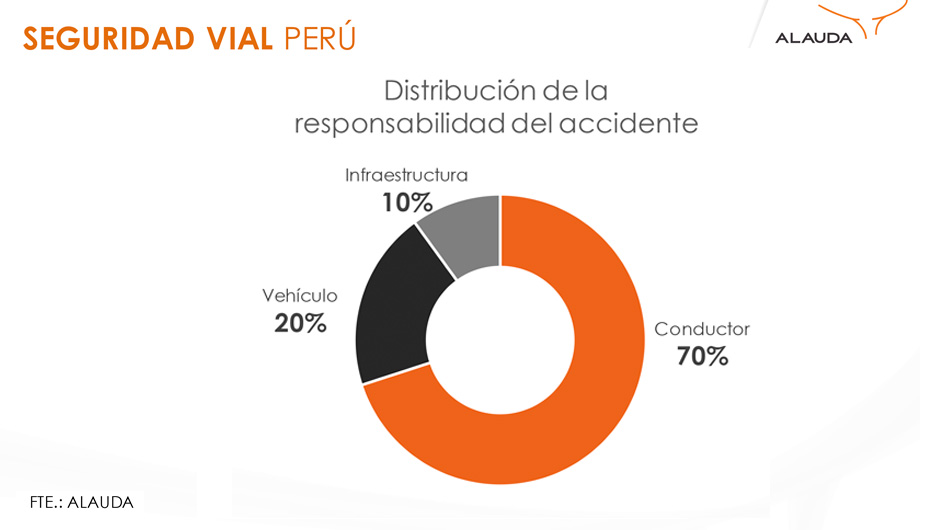
\includegraphics[width=0.5\textwidth]{images/intro/responsabilidad_cond}
	\end{center}
	\begin{center}
	\vskip -0.2cm
	\caption{\small{Análisis de responsabilidad de accidentes}}
	{\small{Fuente acceso: \citep{Gestion1}}}
	\end{center}
	\vspace{-1.5em}
	\end{figure}

	\begin{figure}[H]
	\begin{center}
	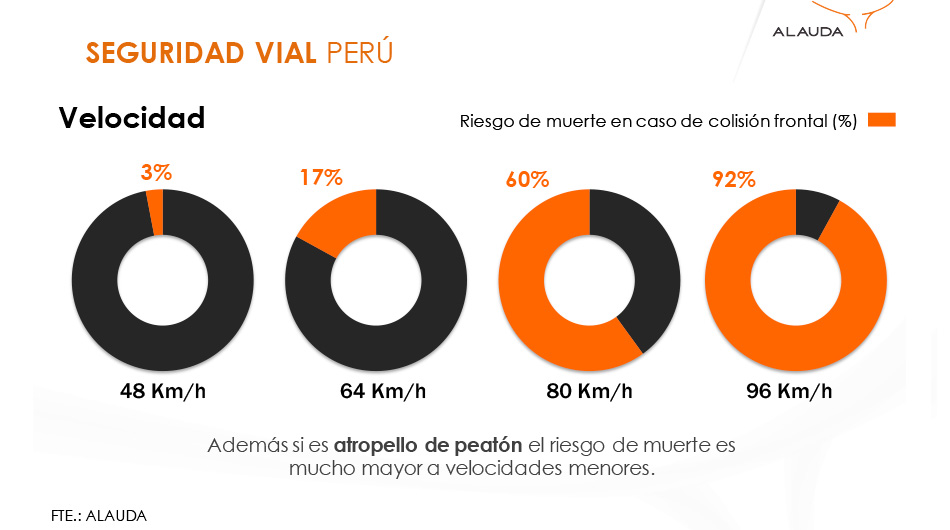
\includegraphics[width=0.6\textwidth]{images/intro/velocidad_ind}
	\end{center}
	\begin{center}
	\caption{\small{Influencia de velocidad en accidentes}}
	{\small{Fuente acceso: \citep{Gestion1}}}
	\end{center}
	\vspace{-1.5em}
	\end{figure}
	
	%Aunque se han publicado algunos estudios sobre este tema, aún no existen comparaciones sistemáticas de enfoques que sean imparciales y no se dispone de conjuntos de datos de referencia completos. 
	
	El reconocimiento de estas señales es un problema de clasificación multicategórica que comúnmente presenta desigualdades en las frecuencias de aparición de las clases. Además, las señales de tránsito muestran una amplia gama de variaciones entre las clases en términos de color, forma y la presencia de símbolos, leyendas o texto. Además, existen subconjuntos de clases (por ejemplo, signos de límite de velocidad) que son muy similares entre sí, lo que representa un reto para el clasificador que tiene que hacer frente a grandes variaciones en las apariencias visuales debido a cambios de iluminación, oclusiones parciales, rotaciones, condiciones meteorológicas, escalamiento, etc.
    

%\%\newpage
\section{Antecedentes de la Investigación}

	En este capítulo se presentan 7 trabajos previos con relación a al tema abordado en la investigación y que sirven de base para este.
	\vskip 0.4cm

	\subsection
	{INTERNACIONALES:}
		\citep{VicenBueno2007} en su paper "Traffic Sign Classification by Image Preprocessing and Neural Networks", propusieron una investigación que se centra en clasificar 9 tipos de señales de tráfico de circulación(color azul) de España utilizando una combinación de diferentes técnicas de preprocesamiento de imágenes junto con una red perceptron de 2 capas la cual produjo un acierto de 98.72\% sobre un conjunto de 78 imágenes para la evaluación. El orden de aplicación de técnicas de preprocesamiento de imágenes es lo más destacable de este antecedente, recomendando usar el filtro mediano para suavizar la imagen, ecualización de histogramas e histogramas vertical y horizontal con un umbral fijo de 185.
		\vskip 0.4cm

		\citep{Rocha2010} en su paper "Sistema de Visión Artificial para la Detección y el Reconocimiento de Señales de Tráfico basado en Redes Neuronales", diseñaron un sistema de detección basado en redes neuronales feedfoward y descriptores de forma conocidos como momentos invariantes. Este sistema fue capaz de entrenarse con algunas señales de tránsito con la meta de asistir al conductor de no cometer una infracción o en el peor de los casos un accidente, reconociendo una señal de tránsito a cierta distancia para que así el conductor a priori tenga el conocimiento de esta. El sistema fue implementado en MATLAB y presentó mejorías frente a sistemas basados en lógica difusa o basados únicamente en procesamiento de imágenes, sin embargo la tasa de acierto no es tan buena obteniéndose un 88.6\% y se recomendó buscar otro método de invarianza que conjuntamente a una red neuronal pueda conseguir mejores resultados. Así el antecedente contribuye a descartar algunos métodos que no puedan presentar mejoras en el reconocimiento de señales de tránsito.
		\vskip 0.4cm

		\citep{Krizhevsky2012} en su investigación """The ImageNet Classification with Deep Convolutional Neural Networks", desarrollaron una red neuronal convolucional grande y profunda para clasificar 1,2 millones de imágenes de alta resolución del concurso ImageNet LSVRC-2010 que categorizaban 1000 clases diferentes de imágenes. Como dato destacable utilizaron un método de regularización muy efectivo para evitar el overfitting de la red denominado dropout, que permitió alcanzar tasas de error mejores que las anteriores técnicas de estado del arte.
		\vskip 0.4cm	

		\citep{Hannan2014} en la investigación realizada en Malasia "Traffic Sign Classification based on Neural Network for Advance Driver Assistance System", elaboraron un sistema con pasos de preprocesamiento y extracción de características para clasificar señales de tránsito usando una red perceptron multicapa que funcione en diferentes condiciones de luminosidad. Lo destacable de la investigación, a parte de que el sistema fue capaz de superar la mayor parte del efecto de iluminación en las imágenes, es el tiempo computacional requerido para el análisis de una imagen, siendo en promedio 0.134s, sin embargo la tasa de precisión no fue buena obteniendose un 84.4\% de acierto para un conjunto de evaluación compuesta por 300 imágenes. 
		\vskip 0.4cm	

		\citep{Hai2014} en su artículo "Morphological Classification for Traffic Sign Recognition", propone un nuevo método para el Reconocimiento de Señales de Tránsito usando el Análisis de Componentes Principales (PCA) y una red Perceptron de Multi-Capa (MLP). En este método propuesto, las señales se detectan individualmente a partir de dos componentes, uno es el color y luego se clasifican en tres clases según la forma: círculo, cuadrado y triángulo. Las características basadas en PCA de estas señales se utilizarán como entrada para la MLP durante la fase de entrenamiento o para responder a clases previamente determinadas. Como contribución resaltante, este enfoque no sólo redujo el tiempo sino que también aumentó el rendimiento en el proceso de reconocimiento. En la simulación, el método propuesto fue evaluado con más de 500 imágenes y su tasa de precisión llegó a cerca del 96\%. 
	\newpage		
	\subsection
	{NACIONALES:}

		\citep{Vargas2015} en su tésis ”Implementación de un Sistema Inteligente para el Reconocimiento de Señales Preventivas de Seguridad vial", desarrolló un sistema basado enteramente en procesamiento de imágenes para la detección y el reconocimiento de señales de tránsito del tipo preventivas, usando para la detección la técnica de segmentación por color y luego un análisis por la forma y posteriormente para el reconocimiento se usó el algoritmo Speed Up Robust Features (SURF). Todo el proceso fue implementado utilizando la herramienta OpenCV, obteniendose un acierto del 88\% en un total de 100 señales evaluadas. De este antecedente se analizará la importancia de introducir la segmentación por color al modelo de reconocimiento que se pretende elaborar.
		\vskip 0.4cm

		\citep{Ayuque2016} en su tésis "Diseño de un sistema de clasificación de señales de tránsito vehicular utilizando redes neuronales convolucionales", diseñó 6 modelos de arquitecturas de redes convolucionales para clasificar diversas señales de tránsito de Alemania, de los cuales el mejor resultado logró un acierto de 95.29\% cerca al estado del arte(99.46\%), en un total de 12630 señales evaluadas. Lo importante del antecendente es que servirá como elemento de comparación para la investigación propuesta. 
		
	\subsection
	{ESTADO DEL ARTE:}

		Para clasificación de señales de tránsito se han realizado diferentes estudios de la base de datos GTSRB (German Traffic Sign Benchmark), que cuenta con más de 50 mil imágenes a color distribuidas en 43 clases.

		\begin{figure}[H]
		\begin{center}
		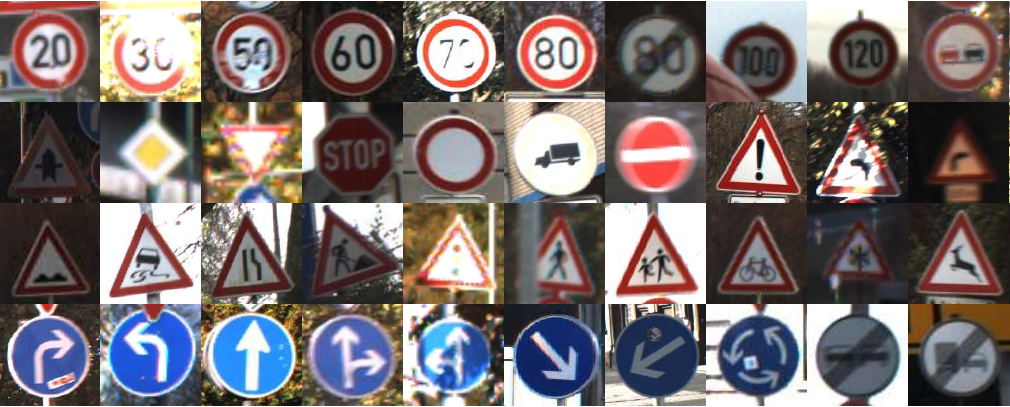
\includegraphics[width=0.7\textwidth]{images/intro/GTSRB}
		\end{center}
		\begin{center}
		\caption{\small{Algunas muestras de la base de datos GTSRB }}
		{\small{Fuente: \citep{Stallkamp2012}}}
		\end{center}
		\vspace{-1.5em}
		\end{figure}
		Estos estudios usan diferentes métodos como Clasificación basado en la Representación Dispersa (Sparse Representation-based Classification), el algoritmo de Vecinos Más Cercanos (Nearest Neightbor Classifier), Máquina de Soporte de Vectores (Support Vector Machine), entre otros. El mejor resultado fue usando una red neuronal convolucional \citep{Ciresan}.
		
		\vskip 0.4cm
		Este conjunto de datos refleja las fuertes variaciones en la apariencia visual de las señales debido a la distancia, la iluminación, las condiciones climáticas, las oclusiones parciales y las rotaciones. Las imágenes se complementan con varios conjuntos de características precalculadas para permitir, de ser necesario, la aplicación de algoritmos de aprendizaje automático sin conocimientos básicos en el procesamiento de imágenes.
		\vskip 0.4cm

		\citep{Ciresan}, utilizó una arquitectura de 9 capas que consistía en una capa de entrada, 3 capas convolucionales usando 100, 150 y 250 filtros cuyos tamaños por cada capa fueron de 42x42, 18x18 y 6x6 neuronas respectivamente, 3 capas pooling con estructuras parecidas a la convolucionales y 1 capa totalmente conectada compuesta por 300 neuronas de entrada para las 43 neuronas de salida que representaban a cada clase.
		\vskip 0.4cm

		Los resultados sobre la base de datos GTSRB fueron realizados a finales del año 2011 produciendo un acierto del 99.46\% para el conjunto de imágenes evaluadas, \citep{Stallkamp2012}; sin embargo, desde el año 2012 se han propuesto nuevas variantes de redes neuronales convolucionales, ya sea usando una funciones de activación diferentes, usando más capas en la red, mas filtros o introduciendo nuevos métodos de optimización.


\section{Formulación del problema}

  En este trabajo, se propone discutir el modelo de redes neuronales convolucionales basado en el problema del reconocimiento de imágenes para responder a la siguiente pregunta:
 \begin{center} 
     ¿Cómo se puede reconocer de manera automática señales de tránsito vehicular?
 \end{center}

\section{Hipótesis}
	 Un modelo basado en el aprendizaje profundo de redes neuronales convolucionales permitirá el reconocimiento automático de señales de tránsito vehicular.

\section{Importancia de la investigación} 

	\subsection{Justificación Académica}

	Recientemente las redes convolucionales profundas han superado los métodos tradicionales de aprendizaje en la clasificación de imágenes. Con los rápidos avances de las estructuras de algoritmos de aprendizaje profundo y la factibilidad de su implementación de alto rendimiento con unidades de procesamiento gráfico (GPU), es ventajoso investigar en problemas de clasificación de imágenes como lo es el reconocimiento de señales de tránsito vehicular desde la perspectiva de un aprendizaje profundo eficiente. Sin embargo realizar esto no es tarea simple, ya que se requiere de un modelo de reconocimiento que funcione para imágenes que se encuentran comúnmente influenciadas por la iluminación, la orientación, la variación de velocidad de los vehículos, entre muchos otros problemas más.  \vskip 0.2cm

	En este sentido esta investigación pretende la elaboración de un modelo basado en el aprendizaje profundo de redes convolucionales que permita el reconocimiento de señales de tránsito vehicular. La siguiente figura muestra un diagrama de bloques con la secuencia de actividades que demanda el reconocimiento.



	\begin{figure}[H]
	\begin{center}
	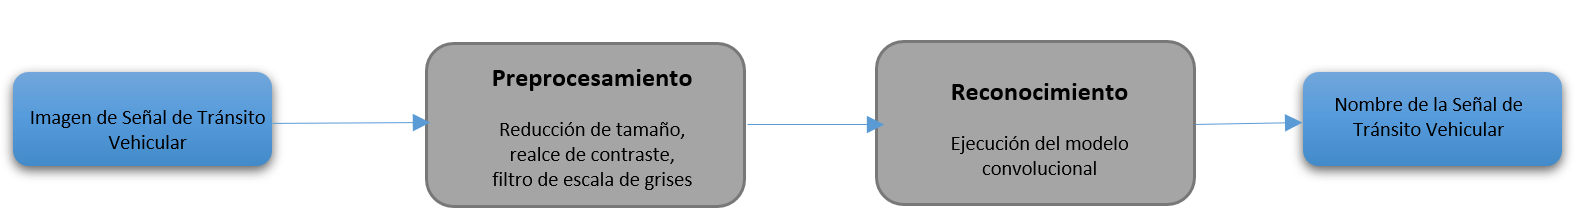
\includegraphics[width=0.8\textwidth]{images/intro/bloque}
	\end{center}
	\begin{center}
	\caption{\small{Diagrama de bloques del modelo prentedido}}
	{\small{Fuente propia}}
	\end{center}
	\vspace{-1.5em}
	\end{figure}


	Por lo tanto, la importancia de esta investigación en el punto de vista de ciencias de la computación se justifica en poner en práctica los conocimientos adquiridos en la formación académica, siendo los más resaltables el tema de procesamiento de imágenes, cálculo matemático e inteligencia artificial con la finalidad de obtener un modelo robusto de redes neuronales convolucionales basadas en el aprendizaje profundo (deep learning) que permita analizar el contenido de imágenes para el reconocer de señales de tránsito vehicular. 


	\subsection{Justificación Social}
	
	Teniendo conocimiento de lo descrito en la realidad problemática, la visibilidad y conocimiento de señales de tráfico es crucial para la seguridad de los conductores y es por ello que la introducción de un modelo de reconocimiento de señales de tránsito que funcione en diferentes contextos puede formar parte de la solución a que constantes infracciones y muertes se puedan evitar y en consecuencia reducir estos indices progresivamente. Por ejemplo, el reconocimiento de estas señales en el momento de la conducción puede ofrecer la posibilidad de dar una notificación al no darse cuenta de un cambio en el límite de velocidad, el aviso de que se está comentiendo una infracción al girar o estacionarse donde no se debe o la advertencia de un peligro potencial por delante. Por otro lado, cuando usuarios desconocen de alguna señal de tránsito, una aplicación móvil que dé la posibilidad de reconocer automáticamente aquella señal serviría como aporte en la educación vial. Adicionalmente, podría ser un componente útil en cámaras de video vigilancia convirtiendolas en más inteligentes con la capacidad de monitorear que las señales de tránsito sean respetadas.\vskip 0.2cm

	Por lo tanto, esta investigación es importante porque a través de un modelo que reconozca señales de tránsito vehicular se contribuye en la industria automotriz, especificamente en los campos de construcción de vehículos autónomos y de los sistemas avanzados de asistencia al conductor(del inglés,ADAS); así como tambíen el modelo pretendido puede ser usado en diferentes plataformas y formar parte de diversos mecanismos que buscan dar soluciones a la inseguridad vial.


\section{Objetivos}
	\subsection{Objetivo general}
	La investigación tiene por objetivo principal implementar un modelo basado en el aprendizaje profundo de redes neuronales convolucionales para reconocer automáticamente señales de tránsito vehicular.
	
	\vskip 0.2cm
		
	\subsection{Objetivos específicos}
	\begin{enumerate}
	
	\item[a)] Obtener un conjunto de imágenes(dataset) donde se muestren diferentes señales de tránsito vehicular.
	\item[b)] Dividir un conjunto de imágenes 2 grupos, uno para el entrenamiento y otro para evaluación y analisar el dataset de entrenamiento a través de métodos de procesamiento de imágenes. De ser necesario, con estos mismos, aumentar la cantidad de imágenes.
	\item[c)] Implementar diferentes arquitecturas de redes convolucionales profundas en las cuales el dataset de entremaniento será procesado.
	\item[d)] Experimentar el uso de diversas funciones de activación, funciones de costo, ajuste de hiperparámetros y métodos de optimización para dichas arquitecturas. 
	\item[e)] Evaluar individualmente el rendimiento que se obtiene de las arquitecturas implementadas en el dataset de entrenamiento y evaluación.
	\item[f)] Elaborar un modelo computacional basado en las evaluaciones realizadas.
	\end{enumerate}

\section{Contribución de la investigación}
	
	Todos los hechos descritos hacen que el reconocimiento de las señales de tránsito sea un reto desafiante y esencial en muchos aspectos, no solo para contribuir en los esfuerzos de la industria automotriz en el campo de la asistencia al conductor, sino también para organismos internacionales y gubernamentales quienes se dan cuenta de la problemática que representa la inseguridad vial y buscan constantemente introducir nuevos mecanismos y tecnologías que faciliten y mejoren la conducción vehicular para el beneficio propio del conductor y en general para la seguridad vial de la sociedad.

\newpage
\section{Metodología de la investigación}
		El desarrollo de la investigación comprenderá las siguientes etapas de trabajo a saber:

		\begin{enumerate}

		\item[a)]	Investigación bibliográfica de los diferentes temas necesarios para la elaboración de la investigación, tales como dispositivos de control de tránsito, vehículos autónomos, sistemas avanzados de asistencia al conductor, aprendizaje profundo (deep learning), procesamiento de imágenes, entre otros.
		
		\item[b)]	Búsqueda de los principales casos de éxito en el reconocimiento de señales de tránsito a tráves de trabajos de investigación en el Perú como tambíen en otros países.

		\item[c)]	Recolección de imágenes de señales de tránsito vehicular que se utilizarán en el desarrollo de la investigación.

		\item[d)]	Análisis e implementación de diversas técnicas de procesamiento de imágenes que serán aplicadas al dataset recolectado con la finalidad de contribuir en el diseño inicial del modelo modelo convolucional.

		\item[e)]	Puesto a que las redes neuronales son heurísticas por naturaleza (requieren un constante ajuste de híper-parámetros para obtener un óptimo resultado), se realizarán diferentes diseños de arquitecturas convolucionales y se escogerá el que otorge los mejores resultados.
		
		\item[f)]	Para el análisis de resultados se pretende usar una Matriz de confusión, en la cual cada fila de la matriz representa las instancias en una clase predecida, mientras que cada columna representa las instancias en una clase real (o viceversa). Además de los indicadores descritos anteriormente(tasa de sensibilidad y de error). Incluso a través de esta matriz se pueden conocer valores estadísticos como el ROC(Receiver Operating Characteristic), métrica usada para evaluar la calidad del modelo clasificador(reconocedor).
		
		\end{enumerate}



\section{Estructura de la tesis}

	\vskip 0.1cm
	El presente trabajo está dividido en seis capítulos. El primer capítulo presenta los aspectos generales del tema tratado: la formulación del problema, importancia de la investigación, los objetivos, la contribución, además de la metodología de la investigación y la estructura de la tesis.

	En el capítulo dos se presenta el referencial teórico, soporte del tema, contemplando los conceptos de inteligencia artificial, aprendizaje automático basado en redes renuronales detallando y diferenciando sus características en el área de aprendizaje profundo. Además se analiza las características y procesos de una red convolucional a detalle.

	El tercer capítulo trata sobre los materiales y las técnicas de recolección de datos

	En el cuarto capítulo es el desarrollo de la tesis, diseñandose los modelos respectivos propuestos y explicando la implementación de cada uno de ellos.
	
	En el quinto capítulo se presentan los resultados obtenidos en la investigación.

	En el capítulo seis se presentan las consideraciones finales obtenidas en esta tesis. Inicialmente se presentan las conclusiones, seguida de las recomendaciones para futuras investigaciones relacionadas al tema en cuestión.

	Finalmente, en el séptimo y octavo capítulo se describen las referencias bibliográficas usadas para la investigación en esta tesis y los anexos donde se presentan los programas elaborados y en apéndice un pequeño glosario de ciertos términos usados en esta investigación.


